\documentclass[twoside]{book}

% Packages required by doxygen
\usepackage{fixltx2e}
\usepackage{calc}
\usepackage{doxygen}
\usepackage[export]{adjustbox} % also loads graphicx
\usepackage{graphicx}
\usepackage[utf8]{inputenc}
\usepackage{makeidx}
\usepackage{multicol}
\usepackage{multirow}
\PassOptionsToPackage{warn}{textcomp}
\usepackage{textcomp}
\usepackage[nointegrals]{wasysym}
\usepackage[table]{xcolor}

% Font selection
\usepackage[T1]{fontenc}
\usepackage[scaled=.90]{helvet}
\usepackage{courier}
\usepackage{amssymb}
\usepackage{sectsty}
\renewcommand{\familydefault}{\sfdefault}
\allsectionsfont{%
  \fontseries{bc}\selectfont%
  \color{darkgray}%
}
\renewcommand{\DoxyLabelFont}{%
  \fontseries{bc}\selectfont%
  \color{darkgray}%
}
\newcommand{\+}{\discretionary{\mbox{\scriptsize$\hookleftarrow$}}{}{}}

% Page & text layout
\usepackage{geometry}
\geometry{%
  a4paper,%
  top=2.5cm,%
  bottom=2.5cm,%
  left=2.5cm,%
  right=2.5cm%
}
\tolerance=750
\hfuzz=15pt
\hbadness=750
\setlength{\emergencystretch}{15pt}
\setlength{\parindent}{0cm}
\setlength{\parskip}{3ex plus 2ex minus 2ex}
\makeatletter
\renewcommand{\paragraph}{%
  \@startsection{paragraph}{4}{0ex}{-1.0ex}{1.0ex}{%
    \normalfont\normalsize\bfseries\SS@parafont%
  }%
}
\renewcommand{\subparagraph}{%
  \@startsection{subparagraph}{5}{0ex}{-1.0ex}{1.0ex}{%
    \normalfont\normalsize\bfseries\SS@subparafont%
  }%
}
\makeatother

% Headers & footers
\usepackage{fancyhdr}
\pagestyle{fancyplain}
\fancyhead[LE]{\fancyplain{}{\bfseries\thepage}}
\fancyhead[CE]{\fancyplain{}{}}
\fancyhead[RE]{\fancyplain{}{\bfseries\leftmark}}
\fancyhead[LO]{\fancyplain{}{\bfseries\rightmark}}
\fancyhead[CO]{\fancyplain{}{}}
\fancyhead[RO]{\fancyplain{}{\bfseries\thepage}}
\fancyfoot[LE]{\fancyplain{}{}}
\fancyfoot[CE]{\fancyplain{}{}}
\fancyfoot[RE]{\fancyplain{}{\bfseries\scriptsize Generated by Doxygen }}
\fancyfoot[LO]{\fancyplain{}{\bfseries\scriptsize Generated by Doxygen }}
\fancyfoot[CO]{\fancyplain{}{}}
\fancyfoot[RO]{\fancyplain{}{}}
\renewcommand{\footrulewidth}{0.4pt}
\renewcommand{\chaptermark}[1]{%
  \markboth{#1}{}%
}
\renewcommand{\sectionmark}[1]{%
  \markright{\thesection\ #1}%
}

% Indices & bibliography
\usepackage{natbib}
\usepackage[titles]{tocloft}
\setcounter{tocdepth}{3}
\setcounter{secnumdepth}{5}
\makeindex

% Hyperlinks (required, but should be loaded last)
\usepackage{ifpdf}
\ifpdf
  \usepackage[pdftex,pagebackref=true]{hyperref}
\else
  \usepackage[ps2pdf,pagebackref=true]{hyperref}
\fi
\hypersetup{%
  colorlinks=true,%
  linkcolor=blue,%
  citecolor=blue,%
  unicode%
}

% Custom commands
\newcommand{\clearemptydoublepage}{%
  \newpage{\pagestyle{empty}\cleardoublepage}%
}

\usepackage{caption}
\captionsetup{labelsep=space,justification=centering,font={bf},singlelinecheck=off,skip=4pt,position=top}

%===== C O N T E N T S =====

\begin{document}

% Titlepage & ToC
\hypersetup{pageanchor=false,
             bookmarksnumbered=true,
             pdfencoding=unicode
            }
\pagenumbering{alph}
\begin{titlepage}
\vspace*{7cm}
\begin{center}%
{\Large My Project }\\
\vspace*{1cm}
{\large Generated by Doxygen 1.8.13}\\
\end{center}
\end{titlepage}
\clearemptydoublepage
\pagenumbering{roman}
\tableofcontents
\clearemptydoublepage
\pagenumbering{arabic}
\hypersetup{pageanchor=true}

%--- Begin generated contents ---
\chapter{File Index}
\section{File List}
Here is a list of all files with brief descriptions\+:\begin{DoxyCompactList}
\item\contentsline{section}{\hyperlink{SolveSquare_8cpp}{Solve\+Square.\+cpp} }{\pageref{SolveSquare_8cpp}}{}
\end{DoxyCompactList}

\chapter{File Documentation}
\hypertarget{SolveSquare_8cpp}{}\section{Solve\+Square.\+cpp File Reference}
\label{SolveSquare_8cpp}\index{Solve\+Square.\+cpp@{Solve\+Square.\+cpp}}
{\ttfamily \#include $<$stdio.\+h$>$}\newline
{\ttfamily \#include $<$math.\+h$>$}\newline
{\ttfamily \#include $<$assert.\+h$>$}\newline
Include dependency graph for Solve\+Square.\+cpp\+:
\nopagebreak
\begin{figure}[H]
\begin{center}
\leavevmode
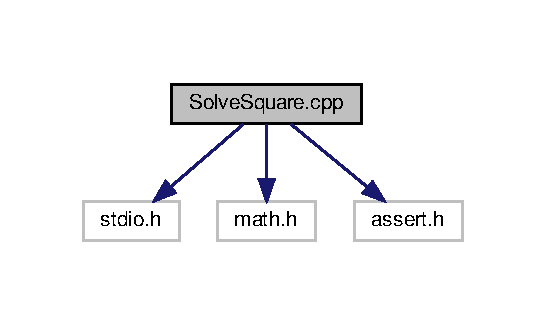
\includegraphics[width=262pt]{SolveSquare_8cpp__incl}
\end{center}
\end{figure}
\subsection*{Macros}
\begin{DoxyCompactItemize}
\item 
\#define \hyperlink{SolveSquare_8cpp_a18d3a495578be1d105cfe11c704a2e17}{S\+E\+\_\+\+I\+N\+F\+\_\+\+R\+O\+O\+TS}~-\/1
\end{DoxyCompactItemize}
\subsection*{Functions}
\begin{DoxyCompactItemize}
\item 
int \hyperlink{SolveSquare_8cpp_ac1ba2f9d576c716484869414f91b7151}{Solve\+Linear} (double a, double b, double $\ast$x)
\item 
int \hyperlink{SolveSquare_8cpp_ab2dd9b24e0e487efdd1cd1f40dd3a023}{Solve\+Square} (double a, double b, double c, double $\ast$x1, double $\ast$x2)
\item 
int \hyperlink{SolveSquare_8cpp_ae66f6b31b5ad750f1fe042a706a4e3d4}{main} ()
\end{DoxyCompactItemize}


\subsection{Macro Definition Documentation}
\mbox{\Hypertarget{SolveSquare_8cpp_a18d3a495578be1d105cfe11c704a2e17}\label{SolveSquare_8cpp_a18d3a495578be1d105cfe11c704a2e17}} 
\index{Solve\+Square.\+cpp@{Solve\+Square.\+cpp}!S\+E\+\_\+\+I\+N\+F\+\_\+\+R\+O\+O\+TS@{S\+E\+\_\+\+I\+N\+F\+\_\+\+R\+O\+O\+TS}}
\index{S\+E\+\_\+\+I\+N\+F\+\_\+\+R\+O\+O\+TS@{S\+E\+\_\+\+I\+N\+F\+\_\+\+R\+O\+O\+TS}!Solve\+Square.\+cpp@{Solve\+Square.\+cpp}}
\subsubsection{\texorpdfstring{S\+E\+\_\+\+I\+N\+F\+\_\+\+R\+O\+O\+TS}{SE\_INF\_ROOTS}}
{\footnotesize\ttfamily \#define S\+E\+\_\+\+I\+N\+F\+\_\+\+R\+O\+O\+TS~-\/1}



\subsection{Function Documentation}
\mbox{\Hypertarget{SolveSquare_8cpp_ae66f6b31b5ad750f1fe042a706a4e3d4}\label{SolveSquare_8cpp_ae66f6b31b5ad750f1fe042a706a4e3d4}} 
\index{Solve\+Square.\+cpp@{Solve\+Square.\+cpp}!main@{main}}
\index{main@{main}!Solve\+Square.\+cpp@{Solve\+Square.\+cpp}}
\subsubsection{\texorpdfstring{main()}{main()}}
{\footnotesize\ttfamily int main (\begin{DoxyParamCaption}{ }\end{DoxyParamCaption})}

\mbox{\Hypertarget{SolveSquare_8cpp_ac1ba2f9d576c716484869414f91b7151}\label{SolveSquare_8cpp_ac1ba2f9d576c716484869414f91b7151}} 
\index{Solve\+Square.\+cpp@{Solve\+Square.\+cpp}!Solve\+Linear@{Solve\+Linear}}
\index{Solve\+Linear@{Solve\+Linear}!Solve\+Square.\+cpp@{Solve\+Square.\+cpp}}
\subsubsection{\texorpdfstring{Solve\+Linear()}{SolveLinear()}}
{\footnotesize\ttfamily int Solve\+Linear (\begin{DoxyParamCaption}\item[{double}]{a,  }\item[{double}]{b,  }\item[{double $\ast$}]{x }\end{DoxyParamCaption})}

Solves a linear equation ax + b = 0


\begin{DoxyParams}[1]{Parameters}
\mbox{\tt in}  & {\em a} & a -\/ coefficient \\
\hline
\mbox{\tt in}  & {\em b} & b -\/ coefficient \\
\hline
\mbox{\tt out}  & {\em x} & Pointer to the root\\
\hline
\end{DoxyParams}
\begin{DoxyReturn}{Returns}
Number of roots
\end{DoxyReturn}
\begin{DoxyNote}{Note}
in case of infinity number of roots, returns S\+E\+\_\+\+I\+N\+F\+\_\+\+R\+O\+O\+TS 
\end{DoxyNote}
\mbox{\Hypertarget{SolveSquare_8cpp_ab2dd9b24e0e487efdd1cd1f40dd3a023}\label{SolveSquare_8cpp_ab2dd9b24e0e487efdd1cd1f40dd3a023}} 
\index{Solve\+Square.\+cpp@{Solve\+Square.\+cpp}!Solve\+Square@{Solve\+Square}}
\index{Solve\+Square@{Solve\+Square}!Solve\+Square.\+cpp@{Solve\+Square.\+cpp}}
\subsubsection{\texorpdfstring{Solve\+Square()}{SolveSquare()}}
{\footnotesize\ttfamily int Solve\+Square (\begin{DoxyParamCaption}\item[{double}]{a,  }\item[{double}]{b,  }\item[{double}]{c,  }\item[{double $\ast$}]{x1,  }\item[{double $\ast$}]{x2 }\end{DoxyParamCaption})}

Solves a linear equation ax$^\wedge$2 + bx + c = 0


\begin{DoxyParams}[1]{Parameters}
\mbox{\tt in}  & {\em a} & a -\/ coefficient \\
\hline
\mbox{\tt in}  & {\em b} & b -\/ coefficient \\
\hline
\mbox{\tt in}  & {\em c} & c -\/ coefficient \\
\hline
\mbox{\tt out}  & {\em x1} & Pointer to the 1st root \\
\hline
\mbox{\tt out}  & {\em x2} & Pointer to the 2st root\\
\hline
\end{DoxyParams}
\begin{DoxyReturn}{Returns}
Number of roots
\end{DoxyReturn}
\begin{DoxyNote}{Note}
in case of infinity number of roots, returns S\+E\+\_\+\+I\+N\+F\+\_\+\+R\+O\+O\+TS 
\end{DoxyNote}

%--- End generated contents ---

% Index
\backmatter
\newpage
\phantomsection
\clearemptydoublepage
\addcontentsline{toc}{chapter}{Index}
\printindex

\end{document}
